\documentclass[12pt,a4paper]{article}
\usepackage[utf8]{inputenc}
\usepackage{CJKutf8}
\usepackage{amsmath}
\usepackage{amsfonts}
\usepackage{amssymb}
\usepackage{graphicx}
\usepackage{booktabs}
\usepackage{array}
\usepackage{tabularx}
\usepackage{longtable}
\usepackage{multirow}
\usepackage{multicol}
\usepackage{xcolor}
\usepackage{float}
\usepackage{geometry}
\usepackage{hyperref}
\usepackage{verbatim}
\usepackage{tikz}
\usepackage{pgfplots}
\pgfplotsset{compat=1.18}
\usetikzlibrary{shapes,arrows,positioning,fit,backgrounds}

% 页面设置
\geometry{left=2.5cm,right=2.5cm,top=2.5cm,bottom=2.5cm}

% 超链接设置
\hypersetup{
    colorlinks=true,
    linkcolor=blue,
    filecolor=magenta,      
    urlcolor=cyan,
}

\title{检索增强推荐系统实验结果}
\author{实验记录}
\date{\today}

\begin{document}
\begin{CJK}{UTF8}{gbsn}

\maketitle

\section{TTARArec模型架构}

\begin{figure}[H]
\centering
\resizebox{\textwidth}{!}{
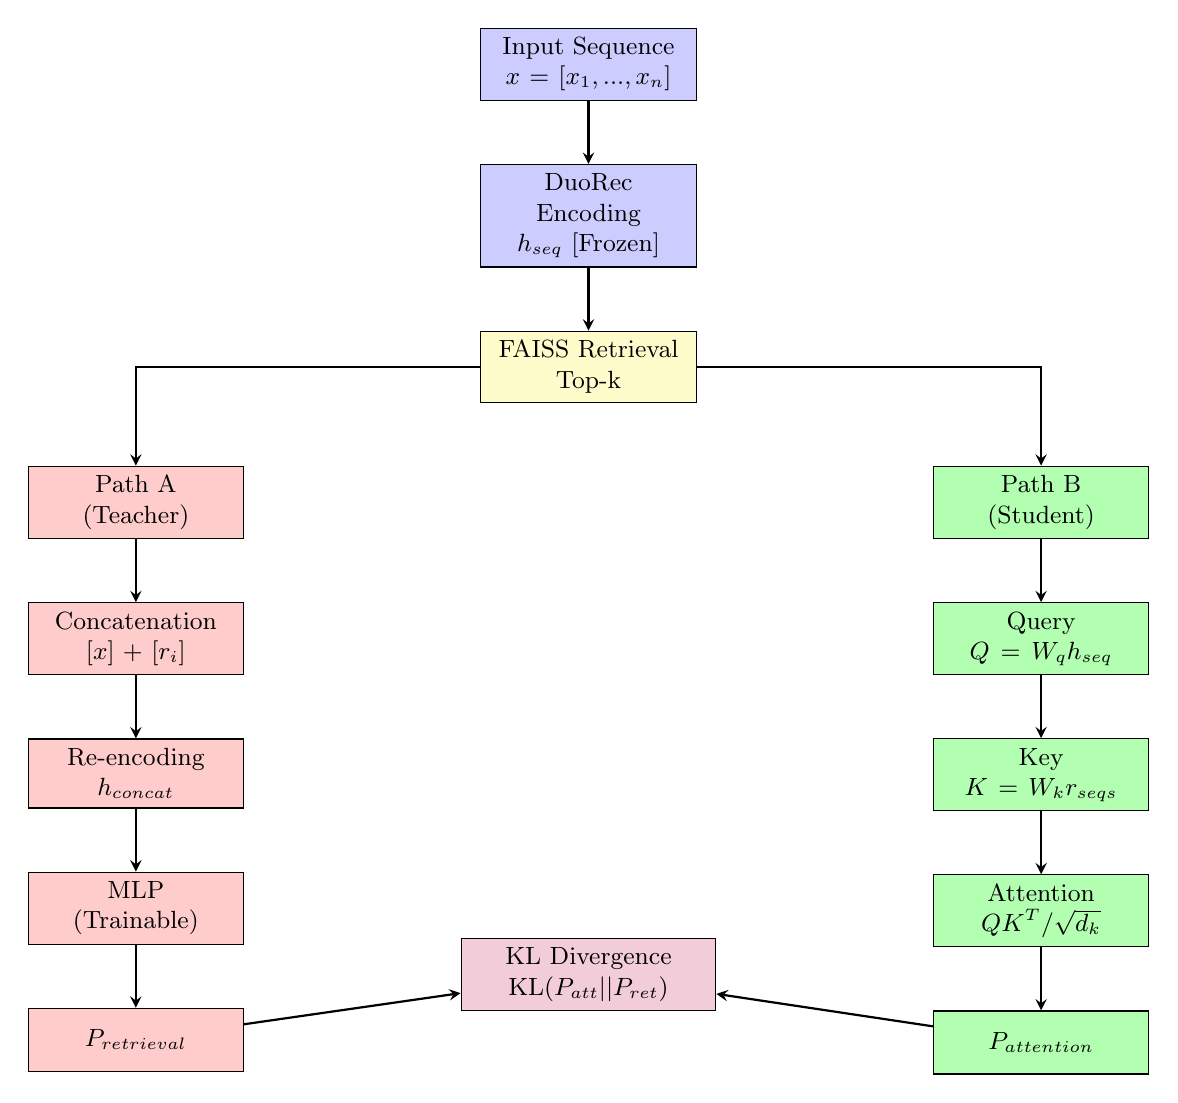
\begin{tikzpicture}[
    node distance=0.8cm and 1.5cm,
    block/.style={rectangle, draw, fill=blue!20, text width=2.5cm, text centered, minimum height=0.8cm, font=\small},
    retrieval/.style={rectangle, draw, fill=red!20, text width=2.5cm, text centered, minimum height=0.8cm, font=\small},
    attention/.style={rectangle, draw, fill=green!30, text width=2.5cm, text centered, minimum height=0.8cm, font=\small},
    kl/.style={rectangle, draw, fill=purple!20, text width=3cm, text centered, minimum height=0.8cm, font=\small},
    arrow/.style={thick,->,>=stealth}
]

% 输入层
\node[block] (input) {Input Sequence\\$x = [x_1, ..., x_n]$};

% DuoRec编码
\node[block, below=of input] (duorec) {DuoRec Encoding\\$h_{seq}$ [Frozen]};

% Faiss检索
\node[block, below=of duorec, fill=yellow!20] (faiss) {FAISS Retrieval\\Top-k};

% 左侧路径：检索分数
\node[retrieval, below left=of faiss, xshift=-1.5cm] (path_a) {Path A\\(Teacher)};
\node[retrieval, below=of path_a] (concat) {Concatenation\\$[x] + [r_i]$};
\node[retrieval, below=of concat] (reencoding) {Re-encoding\\$h_{concat}$};
\node[retrieval, below=of reencoding] (mlp) {MLP\\(Trainable)};
\node[retrieval, below=of mlp] (retrieval_probs) {$P_{retrieval}$};

% 右侧路径：注意力分数
\node[attention, below right=of faiss, xshift=1.5cm] (path_b) {Path B\\(Student)};
\node[attention, below=of path_b] (query_trans) {Query\\$Q = W_q h_{seq}$};
\node[attention, below=of query_trans] (key_trans) {Key\\$K = W_k r_{seqs}$};
\node[attention, below=of key_trans] (attn_comp) {Attention\\$QK^T/\sqrt{d_k}$};
\node[attention, below=of attn_comp] (attention_probs) {$P_{attention}$};

% KL散度对齐
\node[kl, below=of faiss, yshift=-6cm] (kl_div) {KL Divergence\\$\text{KL}(P_{att} || P_{ret})$};

% 连接线
\draw[arrow] (input) -- (duorec);
\draw[arrow] (duorec) -- (faiss);
\draw[arrow] (faiss) -| (path_a);
\draw[arrow] (path_a) -- (concat);
\draw[arrow] (concat) -- (reencoding);
\draw[arrow] (reencoding) -- (mlp);
\draw[arrow] (mlp) -- (retrieval_probs);

\draw[arrow] (faiss) -| (path_b);
\draw[arrow] (path_b) -- (query_trans);
\draw[arrow] (query_trans) -- (key_trans);
\draw[arrow] (key_trans) -- (attn_comp);
\draw[arrow] (attn_comp) -- (attention_probs);

\draw[arrow] (retrieval_probs) -- (kl_div);
\draw[arrow] (attention_probs) -- (kl_div);

\end{tikzpicture}
}
\caption{TTARArec模型架构：KL散度对齐机制}
\label{fig:model_architecture}
\end{figure}

\subsection{模型架构说明}

TTARArec模型采用双路径架构，通过KL散度损失实现注意力评分与检索评分的对齐：

\textbf{核心思想}：让注意力机制学习检索评分的索引选择模式，从而识别真正有用的检索索引。

\textbf{左侧路径（检索评分 - 教师信号）}：
\begin{itemize}
    \item 将原始序列与每个检索序列拼接
    \item 通过冻结的DuoRec重新编码获得增强表征
    \item 使用可训练的MLP层处理表征
    \item 计算与正样本项目的相似度作为检索评分
\end{itemize}

\textbf{右侧路径（注意力评分 - 学生网络）}：
\begin{itemize}
    \item 使用交叉注意力机制计算原始序列与检索序列的注意力权重
    \item Query来自原始序列表征，Key来自检索序列表征
    \item 通过可训练的Query/Key变换矩阵学习注意力模式
\end{itemize}

\textbf{KL散度对齐}：
\begin{itemize}
    \item $L_{KL} = \text{KL}(P_{attention} || P_{retrieval})$
    \item 强制注意力分布向检索分布对齐
    \item 更新参数：检索器MLP + 交叉注意力Query/Key矩阵
\end{itemize}

% 1.2 详细网络结构
\subsection{详细网络结构}
\begin{verbatim}
(pretrained_model): DuoRec(
    (item_embedding): Embedding(12102, 64, padding_idx=0)
    (position_embedding): Embedding(50, 64)
    (trm_encoder): TransformerEncoder(
      (layer): ModuleList(
        (0-1): 2 x TransformerLayer(
          (multi_head_attention): MultiHeadAttention(
            (query): Linear(in_features=64, out_features=64, bias=True)
            (key): Linear(in_features=64, out_features=64, bias=True)
            (value): Linear(in_features=64, out_features=64, bias=True)
            (attn_dropout): Dropout(p=0.5, inplace=False)
            (dense): Linear(in_features=64, out_features=64, bias=True)
            (LayerNorm): LayerNorm((64,), eps=1e-12, elementwise_affine=True)
            (out_dropout): Dropout(p=0.5, inplace=False)
          )
          (feed_forward): FeedForward(
            (dense_1): Linear(in_features=64, out_features=256, bias=True)
            (dense_2): Linear(in_features=256, out_features=64, bias=True)
            (LayerNorm): LayerNorm((64,), eps=1e-12, elementwise_affine=True)
            (dropout): Dropout(p=0.5, inplace=False)
          )
        )
      )
    )
    (LayerNorm): LayerNorm((64,), eps=1e-12, elementwise_affine=True)
    (dropout): Dropout(p=0.5, inplace=False)
    (loss_fct): CrossEntropyLoss()
    (aug_nce_fct): CrossEntropyLoss()
    (sem_aug_nce_fct): CrossEntropyLoss()
)
(retriever_act_fn): GELU(approximate='none')
(retriever_dropout_layer): Dropout(p=0, inplace=False)
(retriever_mlp): ModuleList()
(retriever_layer_norms): ModuleList()
(seq_tar_fusion): CrossMultiHeadAttention(
    (query): Linear(in_features=64, out_features=64, bias=True)
    (key): Linear(in_features=64, out_features=64, bias=True)
    (value): Linear(in_features=64, out_features=64, bias=True)
    (attn_dropout): Dropout(p=0.5, inplace=False)
    (dense): Linear(in_features=64, out_features=64, bias=True)
    (LayerNorm): LayerNorm((64,), eps=1e-12, elementwise_affine=True)
    (out_dropout): Dropout(p=0.5, inplace=False)
)
(fusion_ffn): FeedForward(
    (dense_1): Linear(in_features=64, out_features=256, bias=True)
    (dense_2): Linear(in_features=256, out_features=64, bias=True)
    (LayerNorm): LayerNorm((64,), eps=1e-12, elementwise_affine=True)
    (dropout): Dropout(p=0.5, inplace=False)
)
(fusion_position_embedding): Embedding(10, 64)
\end{verbatim}

\begin{figure}[H]
\centering
\resizebox{\textwidth}{!}{
\begin{tikzpicture}[
    node distance=0.9cm and 1.6cm,
    blk/.style={rectangle, draw, fill=blue!15, rounded corners, minimum width=2.9cm, minimum height=0.9cm, align=center, font=\small},
    attn/.style={rectangle, draw, fill=green!20, rounded corners, minimum width=3.2cm, minimum height=0.9cm, align=center, font=\small},
    ffn/.style={rectangle, draw, fill=orange!20, rounded corners, minimum width=3.2cm, minimum height=0.9cm, align=center, font=\small},
    data/.style={rectangle, draw, fill=gray!10, rounded corners, minimum width=2.6cm, minimum height=0.8cm, align=center, font=\small},
    arrow/.style={thick,->,>=stealth}
]

% 左：DuoRec 编码器
\node[data] (inp) {item\_seq};
\node[blk, below=of inp] (emb) {item/pos Embedding};
\node[blk, below=of emb] (trm1) {TransformerLayer\,\#1};
\node[blk, below=of trm1] (trm2) {TransformerLayer\,\#2};
\node[blk, below=of trm2] (ln) {LayerNorm + Dropout};
\node[data, below=of ln] (hseq) {$h_{seq}$};

\draw[arrow] (inp) -- (emb);
\draw[arrow] (emb) -- (trm1);
\draw[arrow] (trm1) -- (trm2);
\draw[arrow] (trm2) -- (ln);
\draw[arrow] (ln) -- (hseq);

% 右：检索候选（抽象表示）
\node[data, right=5.2cm of trm1] (rseqs) {retrieved\_seqs [B,K,H]};
\node[data, below=of rseqs] (rtars) {retrieved\_tars [B,K,H]};

% 交叉注意力 + FFN
\node[attn, below=0.4cm of hseq, right=3.4cm of hseq] (xattn) {CrossMultiHeadAttention\\(Q=h\_{seq}, K=r\_{seqs}, V=r\_{tars})};
\node[ffn, below=of xattn] (ffn) {FeedForward (256) \rightarrow 64};
\node[data, below=of ffn] (hout) {$h_{aug}$};

\draw[arrow] (hseq.east) -- (xattn.west);
\draw[arrow] (rseqs.west) -- (xattn.north east);
\draw[arrow] (rtars.west) -- (xattn.south east);
\draw[arrow] (xattn) -- (ffn);
\draw[arrow] (ffn) -- (hout);

\end{tikzpicture}
}
\caption{TTARArec 模块级网络结构示意图}
\label{fig:ttara_module_graph}
\end{figure}

\subsection{可训练参数}
\begin{verbatim}
===== 可训练参数列表（requires_grad=True） =====
- seq_tar_fusion.query.weight: shape=(64, 64)
- seq_tar_fusion.query.bias: shape=(64,)
- seq_tar_fusion.key.weight: shape=(64, 64)
- seq_tar_fusion.key.bias: shape=(64,)
- seq_tar_fusion.value.weight: shape=(64, 64)
- seq_tar_fusion.value.bias: shape=(64,)
- seq_tar_fusion.dense.weight: shape=(64, 64)
- seq_tar_fusion.dense.bias: shape=(64,)
- seq_tar_fusion.LayerNorm.weight: shape=(64,)
- seq_tar_fusion.LayerNorm.bias: shape=(64,)
- fusion_ffn.dense_1.weight: shape=(256, 64)
- fusion_ffn.dense_1.bias: shape=(256,)
- fusion_ffn.dense_2.weight: shape=(64, 256)
- fusion_ffn.dense_2.bias: shape=(64,)
- fusion_ffn.LayerNorm.weight: shape=(64,)
- fusion_ffn.LayerNorm.bias: shape=(64,)
- fusion_position_embedding.weight: shape=(10, 64)
总参数量: 928448, 可训练参数量: 50624

[Check] Attention关键参数可训练标记：
  seq_tar_fusion.query.weight: requires_grad=True, shape=(64, 64)
  seq_tar_fusion.query.bias: requires_grad=True, shape=(64,)
  seq_tar_fusion.key.weight: requires_grad=True, shape=(64, 64)
  seq_tar_fusion.key.bias: requires_grad=True, shape=(64,)
  seq_tar_fusion.value.weight: requires_grad=True, shape=(64, 64)
  seq_tar_fusion.value.bias: requires_grad=True, shape=(64,)

\end{verbatim}

\section{融合索引后性能和KL散度对齐效果（核心问题）}

核心思想是让推荐损失给v矩阵传递信号，kl散度给qk传递信号，kl散度损失告诉attention层选什么索引，推荐损失告诉attention层如何用好选择的索引


% 跨数据集模型对比（Recall）
\subsection{模型性能对比（Recall / NDCG）}
% Beauty 表
\begin{table}[H]
\centering
\caption{旧版融合target(Beauty)}
\begin{tabular}{lcccc}
\toprule
\midrule
Dataset & \multicolumn{4}{c}{Beauty} \\
指标 & recall@5 & recall@50 & ndcg@5 & ndcg@50 \\
DuoRec & 0.0537 & 0.1766 & 0.0342 & 0.0637 \\
RaSeRec & 0.0566 & 0.1794 & 0.0358 & 0.0653 \\
TTARArec & 0.0566 & 0.1832 & 0.0362 & 0.0665 \\
TTARArec较DuoRec提升（\%） & 5.40\% & 3.74\% & 5.85\% &s 4.39\% \\
\bottomrule
\end{tabular}
\label{tab:beauty_compare_metrics}
\end{table}

% Sport 表
\begin{table}[H]
\centering
\caption{旧版融合target(Sports)}
\begin{tabular}{lcccc}
\toprule
\midrule
Dataset & \multicolumn{4}{c}{Sport} \\
指标 & recall@5 & recall@50 & ndcg@5 & ndcg@50 \\
DuoRec & 0.0305 & 0.1094 & 0.0189 & 0.0377 \\
RaSeRec & 0.0319 & 0.1116 & 0.0196 & 0.0385 \\
TTARArec & 0.0327 & 0.1148 & 0.0200 & 0.0394 \\
TTARArec较DuoRec提升（\%） & 7.21\% & 4.94\% & 5.82\% & 4.51\% \\
\bottomrule
\end{tabular}
\label{tab:sport_compare_metrics}
\end{table}

% 改为拼接融合序列/检索评分对齐bpr实验结果
\begin{table}[H]
\centering
\caption{改为拼接融合序列/检索评分对齐bpr - Beauty数据集}
\begin{tabular}{lcccccc}
  \toprule
  指标 & recall@5 & recall@10 & recall@50 & ndcg@5 & ndcg@10 & ndcg@50 \\
  \midrule
  Gru4rec & 0.0398 & 0.0619 & 0.1466 & 0.0261 & 0.0332 & 0.0517 \\
  DuoRec & 0.0537 & 0.0816 & 0.1766 & 0.0342 & 0.0431 & 0.0637 \\
  RaSeRec & 0.0566 & 0.0834 & 0.1794 & 0.0358 & 0.0450 & 0.0653 \\
  TTARArec & 0.0550 & 0.0838 & 0.1830 & 0.0360 & 0.0452 & 0.0665 \\
  TTARArec较DuoRec提升（\%） & 2.42\% & 2.69\% & 3.62\% & 5.26\% & 4.87\% & 4.39\% \\
  best & 0.0553 & 0.0852 & 0.1846 & 0.0365 & 0.0460 & 0.0678 \\
  \bottomrule
\end{tabular}
\label{tab:beauty_concat_fusion_metrics}
\end{table}

\begin{table}[H]
  \centering
  \caption{改为拼接融合序列/检索评分对齐bpr - Sport数据集}
  \begin{tabular}{lcccccc}
    \toprule
    指标 & recall@5 & recall@10 & recall@50 & ndcg@5 & ndcg@10 & ndcg@50 \\
    \midrule
    Gru4rec & 0.0220 & 0.0360 & 0.0911 & 0.0142 & 0.0187 & 0.0305 \\
    DuoRec & 0.0304 & 0.0471 & 0.1126 & 0.0186 & 0.0240 & 0.0381 \\
    RaSeRec & 0.0301 & 0.0463 & 0.1122 & 0.0193 & 0.0244 & 0.0387 \\
    TTARArec & 0.0315 & 0.0478 & 0.1150 & 0.0199 & 0.0252 & 0.0397 \\
    TTARArec较DuoRec提升（\%） & 3.61\% & 1.48\% & 2.13\% & 7.00\% & 5.00\% & 4.20\% \\
    \bottomrule
  \end{tabular}
  \label{tab:sport_concat_fusion_metrics}
  \end{table}

% 不同检索评分对比（Beauty）
\begin{table}[H]
\centering
\caption{不同检索评分对比（Beauty）}
\begin{tabular}{lcccccc}
\toprule
方法 & recall@5 & recall@10 & recall@50 & ndcg@5 & ndcg@10 & ndcg@50 \\
\midrule
对齐BPRLoss & 0.0543 & 0.0843 & 0.1846 & 0.0358 & 0.0455 & 0.0673 \\
正样本相似度 & 0.0535 & 0.0841 & 0.1840 & 0.0356 & 0.0455 & 0.0673 \\
正样本相似度为负 & 0.0537 & 0.0839 & 0.1828 & 0.0358 & 0.0455 & 0.0669 \\
正负样本差分 & 0.0552 & 0.0843 & 0.1836 & 0.0357 & 0.0451 & 0.0667 \\
margin函数优化排序 & 0.0546 & 0.0838 & 0.1821 & 0.0357 & 0.0451 & 0.0665 \\
margin（共享负样本） & 0.0553 & 0.0847 & 0.1838 & 0.0359 & 0.0454 & 0.0669 \\
\bottomrule
\end{tabular}
\label{tab:beauty_retrieval_scores_compare}
\end{table}

% 不同拼接方式对比（Beauty）
\begin{table}[H]
\centering
\caption{不同拼接方式对比（Beauty）}
\small
\setlength{\tabcolsep}{4pt}
\resizebox{\textwidth}{!}{
\begin{tabular}{lcccccc}
\toprule
方法 & r@5 & r@10 & r@50 & n@5 & n@10 & n@50 \\
\midrule
(1) 固定target拼接 & 0.0553 & 0.0847 & 0.1838 & 0.0359 & 0.0454 & 0.0669 \\
(2) 重叠top-1拼接下一item & 0.0544 & 0.0830 & 0.1801 & 0.0345 & 0.0436 & 0.0647 \\
(3) 全局最重叠部分拼接 & 0.0529 & 0.0805 & 0.1799 & 0.0343 & 0.0432 & 0.0648 \\
(4) 用taritem替末尾 & 0.0551 & 0.0841 & 0.1837 & 0.0364 & 0.0457 & 0.0674 \\
(5) 用检索q末项替原末尾 & 0.0549 & 0.0832 & 0.1806 & 0.0350 & 0.0441 & 0.0653 \\
(7) 表征加权混合 & 0.0537 & 0.0821 & 0.1782 & 0.0340 & 0.0432 & 0.0641 \\
(8) 拼接+MLP回64维 & 0.0528 & 0.0820 & 0.1784 & 0.0339 & 0.0433 & 0.0643 \\
\bottomrule
\end{tabular}}
\label{tab:beauty_concat_method_compare}
\end{table}





% 新增：KL散度量纲说明
\subsection{kl散度量纲}
\paragraph{初始损失组成（示例）}
\begin{itemize}
    \item 推荐损失: 6.841918
    \item KL散度损失: 0.483760
    \item 总损失: 1.755392
\end{itemize}

\paragraph{量纲与计算说明}
\begin{itemize}
    \item KL散度与交叉熵均为\textbf{无量纲}（信息量，常以\emph{nats}表示），因此可以线性加权相加。数值尺度与类别数/候选数有关：例如 K=10 时，$\ln K\approx2.303$。
    \item 本实现中使用 \texttt{F.kl\_div(log\_attention\_probs, teacher\_probs, reduction='batchmean')}：对类别维（K）\textbf{求和}后，再对 batch 维\textbf{取均值}，得到标量 KL 损失。
    \item 推荐损失（全排序交叉熵）的典型初始量级约为 $\mathcal{O}(\ln N)$（N为物品数），KL 的量级约为 $\mathcal{O}(\ln K)$，两者通过权重进行平衡。
    \item 推荐损失（交叉熵损失CE）：先计算全物品相似度，然后再 softmax 得到每个物品概率，最后拿正样本概率做 $-\log p(i, y_i)$ 得到该样本损失，最后平均 batch，6.7 的平均损失说明在全库上正样本概率在 0.0011 左右
    \item KL 散度损失：先 $qk/\sqrt{k}$ 做 softmax 得到融合概率，然后将索引融合编码得到的表征做相似度得到 logits 后 softmax 得到概率，将两个概率做 KL 散度计算得到损失，理论上限是 $\ln(k)$。
    \item 回合损失：KL 损失和推荐损失加权和，再乘 batch 的数量
  \end{itemize}
\section{实验结果记录}
\end{CJK}
\end{document}

